\documentclass[12pt]{article}

\usepackage [margin = 1 in] {geometry}
\usepackage [utf8] {inputenc}
\usepackage {amsmath}
\usepackage {fancyhdr}
\usepackage {setspace}
\usepackage {csquotes}
\usepackage {graphicx}
\usepackage {float}

\title {Analogical Reasoning in Foreign Policy Decision-Making}
\author {Sudhan Chitgopkar
  \and Sydney Buchanan
  \and Sarah Wakeman
  \and Sophia Hanchey}
\date {}

\pagestyle {fancy}
\lhead {Group Elle Driver}
\chead {Role of Analogies in Foreign Pol.}
\rhead {\today}

\setlength {\parindent} {0 pt}
\doublespacing

\begin {document}
\tableofcontents
\newpage
\section {Introduction \& Question}
Analogical reasoning, though sometimes considered trivial, may play a nuanced role in decision-making. Understanding the effects of analogical reasoning is therefore critical to a complete understanding of foreign policy decision-making. Contemporary literature on the subject indicates that analogies serve to define an entire context, constrain a decision maker’s win-set, and fundamentally affect an individual’s understanding of a situation. To further understand this phenomenon, this study investigates the role of analogical reasoning in altering individuals’ foreign policy opinions towards artificial intelligence (AI) weapon development. The core research question proposed is as follows:
\begin{center}
\textit{Can the use of an analogy affect an individual’s opinion \\ towards the development of U.S AI weaponry?}
\end{center}
This study provides participants with a brief research vignette regarding U.S. AI weapon development and analyzes whether the inclusion of an analogy in the vignette affects individual opinion.
\section {Literature Review}
As previously mentioned, contemporary literature discusses the effects of analogical reasoning on foreign policy decision-making. Firstly, the literature defines analogies as “shortcuts that are used to compare one thing to another” (Houghton 1996). Interestingly, there is widespread agreement amongst cognitive decision-making scholars that analogical reasoning is an innate function of the human brain. Accordingly, humans often rely on analogies to simplify complex problems and situations.
\bigbreak
Analogical reasoning also seems to be an effective method to make sense of novel scenarios (Houghton 1996). Because analogies allow people to understand an issue and develop a framework for future action, they are effective in providing direction during unfamiliar situations (Houghton 1996, Khong 1992). Specifically, analogies are effective in providing actors a framework of (1) which strategies will and will not be effective responses to a given situation, and (2) the potential risks of action or inaction. The use of analogical reasoning in novel situations should be approached cautiously, though. Because novel situations are, by definition, unprecedented, few analogies are likely to be applicable. This is problematic, as the application of an ill-fitting analogy to a novel foreign policy situation will likely yield a malformed incentive structure that does not properly consider the effects of each strategy.
\bigbreak
Decision makers also use analogies to legitimize and support an already-made policy decision (Taylor and Rourke 1995). Consequently, analogies have the potential to be powerful foreign policy tools during crisis decision-making.
\bigbreak
Importantly, the literature does not address all questions regarding the effects of analogical reasoning in foreign policy. More specifically, it doesn’t quantify how useful analogical reasoning may be in preemptively creating support for foreign policy endeavors, nor does it explain how severe an analogy must be for it to be effective in influencing actors’ decisions.
\section {Significance}
This study builds off the aforementioned literature to better understand how analogies affect decision-making. The significance of this study is three-fold. Firstly, existing literature points towards the potential for analogies to be used as a means of shaping public opinion (Risdianto 2016). A robust understanding of the effects of analogical reasoning in this regard is particularly important, as shifting public opinion may allow decision-makers to alter their win-set. More specifically, if a decision-maker can use analogies to sway public opinion in a particular direction, they may be able to open up their win-set and pursue a policy that may not have been possible otherwise. 
\bigbreak
Second and more importantly, the use of inaccurate analogies may be used by leaders to make disastrous foreign policy decisions. Empirical examples of this are rife, with the literature pointing to the failed Bay of Pigs Invasion (Murgado 2009) and the Iranian Hostage Crisis (Houghton 1996) as specific case studies. In the pursuit of minimizing the number of harmful foreign policy decisions made as a result of improper analogical reasoning, this study hopes to add to existing research.
\bigbreak
Finally, understanding the use of analogical reasoning with respect to AI specifically is critical. As the number of Internet of Things (IoT) devices boom (Burhan et al 2018), the AI industry’s market share has been increasing exponentially (IDC 2021). Given the seemingly endless military and civilian applications of AI, it is likely that global familiarity with the topic will increase dramatically. Problematically, the field of AI is highly technical and understandably difficult to access for most. As a result, it stands to reason that analogies explaining AI technology will be extremely prevalent. In this regard, the results of this study have critical implications for foreign policy decisions on AI technology moving forward.
\section {Theory}
Given the findings of related studies, it is predicted that support for U.S. AI weaponry development will decrease when a negative analogy is applied. Because this study uses an analogy that paints A.I weaponry as primitive and potentially disastrous, it is expected that the opinions of participants in the treatment group will shift against A.I weaponry development. Since existing literature finds that analogical reasoning can have a strong effect on foreign policy opinions, it is expected that the results of this study will be statistically significant.
\section {Research Design}
This experiment was conducted using a between-subjects design, with one group receiving a control vignette and the other receiving a treatment vignette. Both the control and treatment vignette (appendix 8.2.1 \& 8.2.2 respectively) included a brief, identical summary of China’s recent AI development and the U.S.’ reaction to it, which reads as follows:

\begin{displayquote}
\textit{Recent intelligence indicates that China is working on integrating artificial intelligence into their weapon systems. Such weaponry could choose its own targets and carry out attacks without any human oversight. The US has accordingly considered developing their own similar AI weaponry. This has left national security advisors sharply divided, with some experts concerned about the war-time decisions AI might make.}
\end {displayquote}
The treatment vignette was identical but also included the following analogy at the end: \textit{“One official noted that developing AI weaponry would be akin to ‘handing a toddler a hand grenade.’”} Participants from both groups were then asked the following question (appendix 8.2.3): \textit{“Should the U.S. develop its own AI weapons systems to combat Chinese AI weaponry?”}
\bigbreak
This study mentions China in the research vignette for two reasons. Firstly, China is currently developing AI technology, making the vignette both more realistic and practical. Second and more importantly, the inclusion of China in the research vignette was intended to bias participants towards supporting the U.S. development of AI technology. Because participants would likely view Chinese weapon development as a threat to U.S. security and interests, they would be more likely to be in favor of U.S. AI weapons development. If the application of the analogy shifts public opinion away from U.S. AI weaponry development despite participants’ pre-existing biases against China, then this experiment will provide even more conclusive evidence for the effects of analogical reasoning in foreign policy decision-making. 
\bigbreak
The data for this experiment were collected in April 2021 via Amazon’s Mechanical Turk. Survey respondents took an average of seven to eight minutes to complete the survey and were compensated two dollars for their time. Participants were randomly assigned to either the control or treatment group, which determined whether or not they received the analogy. Once the results of the survey were received, the data were quantified by converting an answer of “No” to zero and an answer of “Yes” to one. These values were then used to conduct an unpaired, one-tailed t-test, and the corresponding p-value was derived to test for statistical significance.
\section {Results \& Implications}
\subsection {Results}
Using the aforementioned research design, this study was conducted using a total of 396 participants. The control group consisted of 193 participants, while the remaining 203 participants composed the treatment group. Of the 193 participants in the control group, 93 responded “No” when asked if they supported U.S. development of A.I. weaponry while 100 participants responded “Yes”. Of the 203 participants in the treatment group (presented with an analogy) 138 responded “No” when asked if they supported the U.S. development of A.I. weaponry and 65 participants responded “Yes”.
\bigbreak
The below table exhibits some relevant statistics from the raw data gathered. 

\begin {table} [!ht]
  \centering
  \begin {tabular} {c|c|c}
    Statistic&Control&Treatment \\
    \hline
    Sample Sizes&193&203 \\
    Mean&0.32&0.52 \\
    Standard Dev.&0.47&0.50 \\
  \end {tabular}
  \caption {Treatment-Control Group Statistics}
\end {table}

An unpaired, one-tailed t-test was conducted to analyze the above described raw data. A t-test is one of the most effective tests to use here, as t-tests compare two means and are generally used to determine whether some treatment had a significant impact on some sample. The t-test is unpaired because each study participant received only one vignette - either the control or the treatment. Finally, a single tail was used as the proposed hypothesis is directional. Because it was hypothesized that use of analogical reasoning would decrease public support for A.I weapons development, rather than just changing public opinion, this hypothesis is directional and a single-tailed test is necessary.
\bigbreak
Using the unpaired, one-tailed t-test, it was observed that the participants presented with an analogy reflected less support for U.S. AI weapon development on average than their control group counterparts. Specifically, The 203 participants presented with an analogy (M=0.52, SD=0.50.) reflected less support for U.S. AI development on average than the 193 participants that were not presented with an analogy (M=0.32, SD=0.47); t(388.488)= 4.44, p$\le$.001. With a t-value of ~4.44 and a corresponding p-value of $\le$ .001, the change in public support was statistically significant. This indicates that the inclusion of an analogy designed to bias survey participants against AI weaponry was effective in decreasing support for U.S. development of such technology. The mathematics supporting the above conducted t-test are referenced as appendix 8.1.
\bigbreak
Indeed, the difference in public opinion can be seen graphically below:
\begin{figure} [H]
\centering
\begin{minipage}{0.5\textwidth}
  \centering
  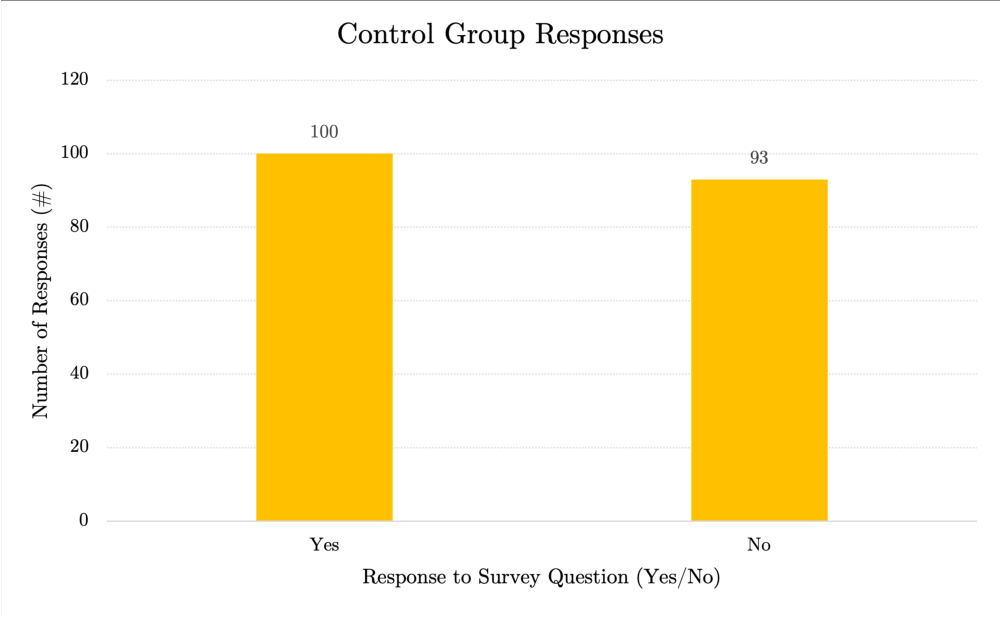
\includegraphics[width=0.9\linewidth]{ControlResponses.pdf}
  \caption{Number of Yes/No Respondents\\in the Control Group}
  \label{fig:test1}
\end{minipage}%
\begin{minipage}{.5\textwidth}
  \centering
  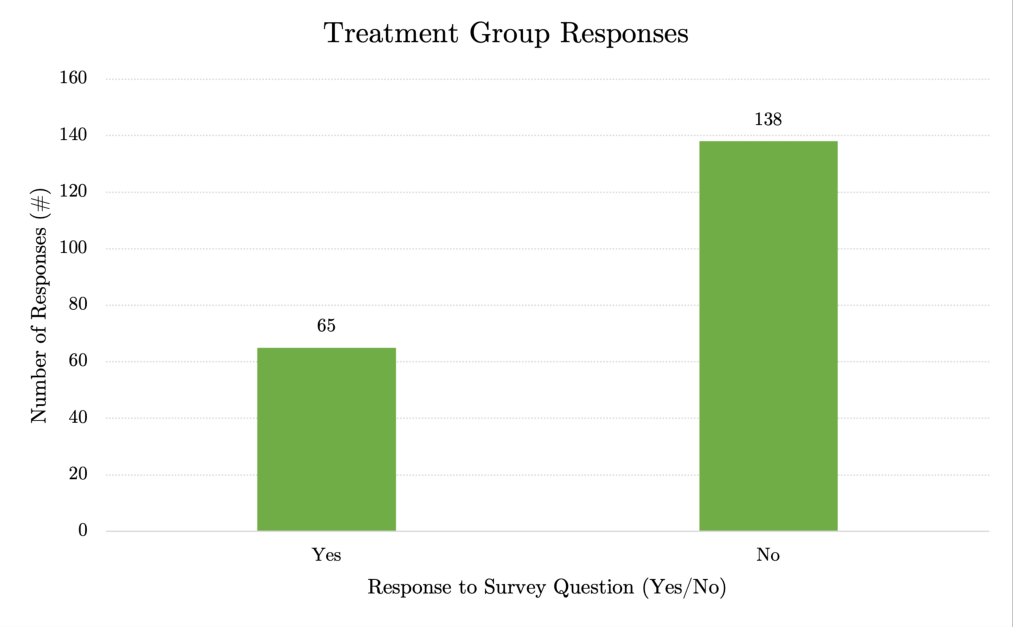
\includegraphics[width=0.9\linewidth]{TreatmentResponses.pdf}
  \caption{Number of Yes/No Respondents\\in the Treatment Group}
  \label{fig:test2}
\end{minipage}
\end{figure}
Observably, there was a significant shift in public opinion towards development of AI weaponry upon application of the treatment. Specifically, the mean response shifted twenty (20) percentage points after treatment application. This, combined with the low standard deviation variation between the control and treatment (observable in table (1)) likely contributed to the small p-value obtained by this study.
\subsection {Implications}
The implications of this positive result are critical. With respect to AI weaponry specifically, the use of a harsh analogy such as the one presented in this paper is likely to affect individuals’ foreign policy prescriptions. More broadly, the positive result of this study confirms pre-existing findings in the literature that document the effects analogies have in foreign policy decision-making. Specifically, analogies may be used by decision-makers to shape or direct public opinions both before and after they make a decision. This allows them to alter the win-set, either opening or constraining it depending on the type of analogy they employ. Furthermore, decision-makers themselves are vulnerable to the effects of analogical reasoning, and may make problematic decisions as a result of an ill-fitting analogy. 
\bigbreak
Though this study produced a positive result, it is important to consider the potential implications of a negative result. As previously mentioned, existing research on the effectiveness of analogies in foreign policy doesn’t clarify how useful analogical reasoning may be in preemptively creating support for foreign policy initiatives. Additionally, it is also easy to employ the use of an ill-fitting analogy when faced with novel situations. Had this experiment produced a negative result, it would have been reasonable to assume that the analogy used in the treatment was ill-fitting, thus failing to elicit a significant response from survey participants.
\newpage
\section {Works Cited}
\begin {enumerate}
  \item Burhan et al. (2018). IoT Elements, Layered Architectures and Security Issues: A Comprehensive Survey. Sensors. 18. 10.3390/s18092796. 

  \item Houghton, David Patrick. “The Role of Analogical Reasoning in Novel Foreign-Policy Situations.” \textit{British Journal of Political Science} 26, no. 4 (1996): 523-52. \texttt{https://doi.org/10.1017/s0007123400007596}.

    \item International Data Corporation. (2021). IDC Forecasts Improved Growth for Global AI Market in 2021. 

    \item Khong, Yuen Foong. Analogies at War: Korea, Munich, Dien Bien Phu, and the Vietnam Decisions of 1965. Princeton, NJ: \textit{Princeton University Press}, 1992

    \item Murgado, Amaury, "The Bay Of Pigs Invasion: A Case Study In Foreign Policy Decision-making" (2009). Electronic Theses and Dissertations, 2004-2019. 4117.\\ \texttt{https://stars.library.ucf.edu/etd/4117}.

    \item Risdianto, Faizal. 2016. The Use of Metaphor in Barack Obama‘s Inauguration Speech. Language Circle: \textit{Journal of Language and Literature}, X/2.

    \item Taylor, Andrew J., and John T. Rourke. “Historical Analogies in the Congressional Foreign Policy Process.” \textit{The Journal of Politics} 57, no. 2 (1995): 460–68.\\ \texttt{https://doi.org/10.2307/2960316}. 

\end {enumerate}
\newpage
\section {Appendix}
\subsection {Significance Calculations}
The general two-sample t-test formula is as follows:
$$t = \frac{\bar{x_a} - \bar{x_b}}{\sqrt{\frac{{S_a}^2}{n_a} + \frac{{S_b}^2}{n_b}}}$$
The conducted experiment yeilded the following raw data:
\begin {table} [!ht]
  \centering
  \begin {tabular} {c|c|c} 
    Statistic&Control&Treatment \\
    \hline
    Sample Sizes&193&203 \\
    Mean&0.32&0.52 \\
    Standard Dev.&0.47&0.50 \\
  \end {tabular}
  \bigbreak
  Table 1 (Copy): Treatment-Control Group Statistics
\end {table}
\smallbreak
Degrees of Freedom = $193 - 1 = 192$.
\bigbreak
Where a is the treatment and b is the control, the following equation is solved for t: 
\begin{align}
t &= \frac{0.52 - 0.32}{\sqrt{\frac{{0.52}^2}{194} + \frac{{0.47}^2}{206}}} \\ 
t &= \frac{0.20}{\sqrt{0.001 + 0.001}} \\
t &= \frac{0.20}{0.045} \\
t &= 4.4\bar{44}
\end{align}
$t$, for a single tail, corresponds to a p-value of $\le .00003$.
\newpage
\subsection {Experimental Text}
\subsubsection {Control}
``Recent intelligence indicates that China is working on integrating artificial intelligence into their weapon systems. Such weaponry could choose its own targets and carry out attacks without any human oversight. The US has accordingly considered developing their own similar AI weaponry. This has left national security advisors sharply divided, with some experts concerned about the war-time decisions AI might make.''
\subsubsection {Treatment}
``Recent intelligence indicates that China is working on integrating artificial intelligence into their weapon systems. Such weaponry could choose its own targets and carry out attacks without any human oversight. The US has accordingly considered developing their own similar AI weaponry. This has left national security advisors sharply divided, with some experts concerned about the war-time decisions AI might make. One official noted that developing AI weaponry would be akin to ‘handing a toddler a hand grenade.’''
\subsubsection {Question}
``Should the U.S. develop its own AI weapons systems to combat Chinese AI weaponry?''
\end {document}
